\documentclass[12pt,a4paper]{article}

\usepackage[a4paper,margin=1in]{geometry}
\usepackage[final]{graphicx}
\graphicspath{{../output_plots/}}
\usepackage{booktabs}
\usepackage{amsmath,amssymb}
\usepackage{float}
\usepackage{hyperref}
\usepackage{xcolor}
\usepackage{listings}
\usepackage{enumitem}
\usepackage{fancyhdr}
\usepackage{longtable}

\hypersetup{colorlinks=true,linkcolor=blue,urlcolor=blue}

\pagestyle{fancy}
\fancyhf{}
\lhead{ICS1512}
\rhead{Machine Learning Algorithms Laboratory}
\cfoot{\thepage}

\lstset{
language=Python,
basicstyle=\ttfamily\small,
numbers=left,
frame=single,
breaklines=true,
showstringspaces=false
}

\begin{document}

\begin{tabular}{|p{4cm}|p{11cm}|}
\hline
Experiment No. & 3 \\ \hline
Experiment Title & Regression Analysis using Linear and Regularized Models
\footnote{\textbf{GitHub Repository: }\url{https://github.com/Danush-k/Machine-Learning}}\\ \hline
Student Name & Danusu K \\ \hline
Register Number & 3122247001013 \\ \hline
Faculty & Dr. Poreddy Ajay Kumar Reddy \\ \hline
Submission Date & \today \\ \hline
\end{tabular}

\section{Objective}
Implement baseline Linear Regression and regularized regression models (Ridge, Lasso, and Elastic Net) to predict a continuous target variable (\texttt{Loan Sanction Amount (USD)}). Evaluate model performance using multiple regression metrics (MAE, MSE, RMSE, $R^2$, and execution time), tune regularization hyperparameters using 5-Fold Cross Validation, generate required visual diagnostics, and analyze overfitting, underfitting, feature sparsity, and bias--variance trade-offs.

\section{Problem Statement}
In financial services, accurately determining the sanctioned loan amount for an applicant based on economic indicators, credit background, and property assets is crucial to manage credit risk and avoid defaults. The objective is to build a predictive regression pipeline on real-world loan application data. Mathematically, given an input feature vector $\mathbf{x} \in \mathbb{R}^d$, we aim to learn a weight vector $\mathbf{w}$ and bias $b$ to estimate the continuous target $y \in \mathbb{R}^+$ (\texttt{Loan Sanction Amount}) by minimizing prediction error subject to regularization penalties.

\section{Dataset Description}
\begin{longtable}{|p{6cm}|p{8cm}|}
\hline
Dataset Name & Predict Loan Amount Data \\ \hline
Dataset Source & Kaggle \\ \hline
Number of Samples & 30000 \\ \hline
Number of Features & 20 (53 post-encoding) \\ \hline
Number of Classes & Continuous Target \\ \hline
Missing Values & 0 (imputed via median/mode) \\ \hline
Train-Test Split & 80\% Train, 20\% Test \\ \hline
\end{longtable}

\section{Exploratory Data Analysis}
Exploratory Data Analysis (EDA) was performed to audit feature properties, target skewness, and predictor relationships:
\begin{itemize}
\item \textbf{Dataset Overview}: Inspected 30,000 raw customer records across 24 initial features.
\item \textbf{Statistical Summary}: Transposed statistical summary of numerical continuous features.
\item \textbf{Missing Value Analysis}: Detected and quantified missing entries across features.
\item \textbf{Class Distribution}: Visualized target variable (\texttt{Loan Sanction Amount (USD)}) spread.
\item \textbf{Correlation Matrix}: Computed feature-target linear correlation coefficients.
\item \textbf{Feature Distribution}: Analyzed bivariate relationships between key predictors and target.
\end{itemize}

\begin{figure}[H]
\centering
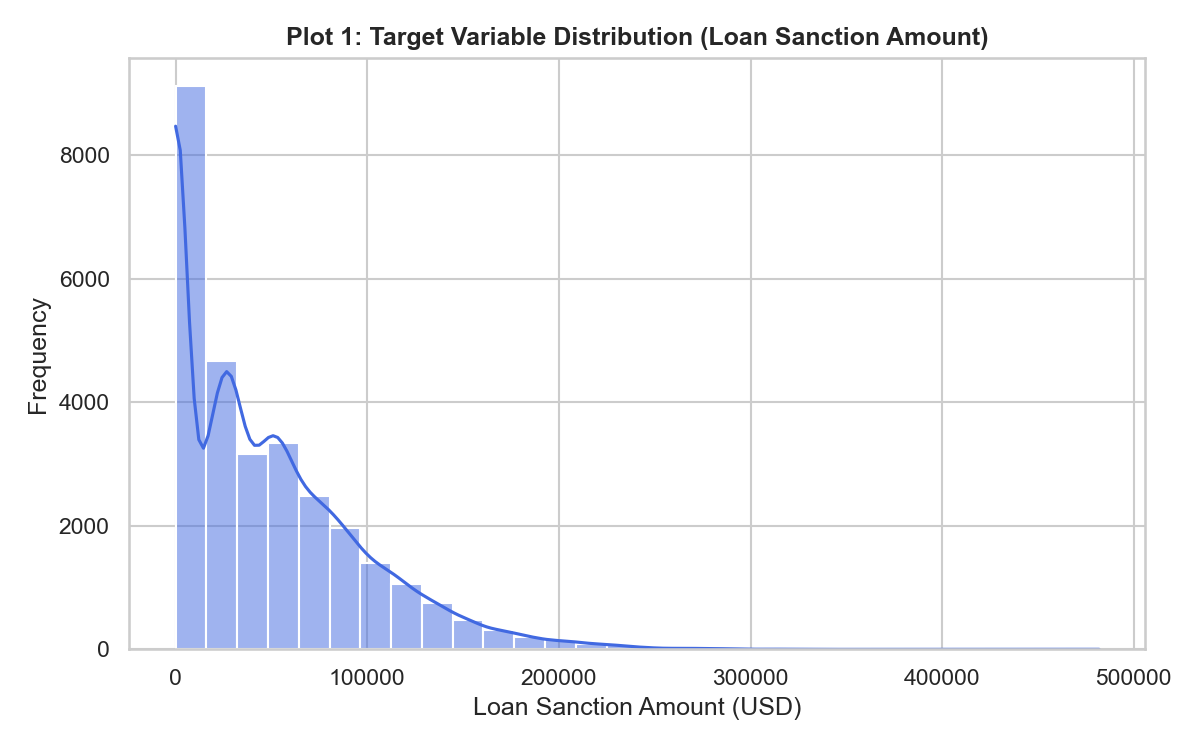
\includegraphics[width=0.65\linewidth]{1_target_distribution.png}
\caption{Distribution of Target Variable (Loan Sanction Amount in USD)}
\label{fig:target_dist}
\end{figure}

\textbf{Inference:}
The target distribution plot shows that \texttt{Loan Sanction Amount (USD)} spans from 0 to over \$400,000, displaying a moderate right-skewed tail with a primary concentration around \$20,000 to \$80,000. Zero values correspond to rejected loan applications. The continuous spread confirms that linear and regularized regression modeling is appropriate for this continuous prediction task.

\begin{figure}[H]
\centering
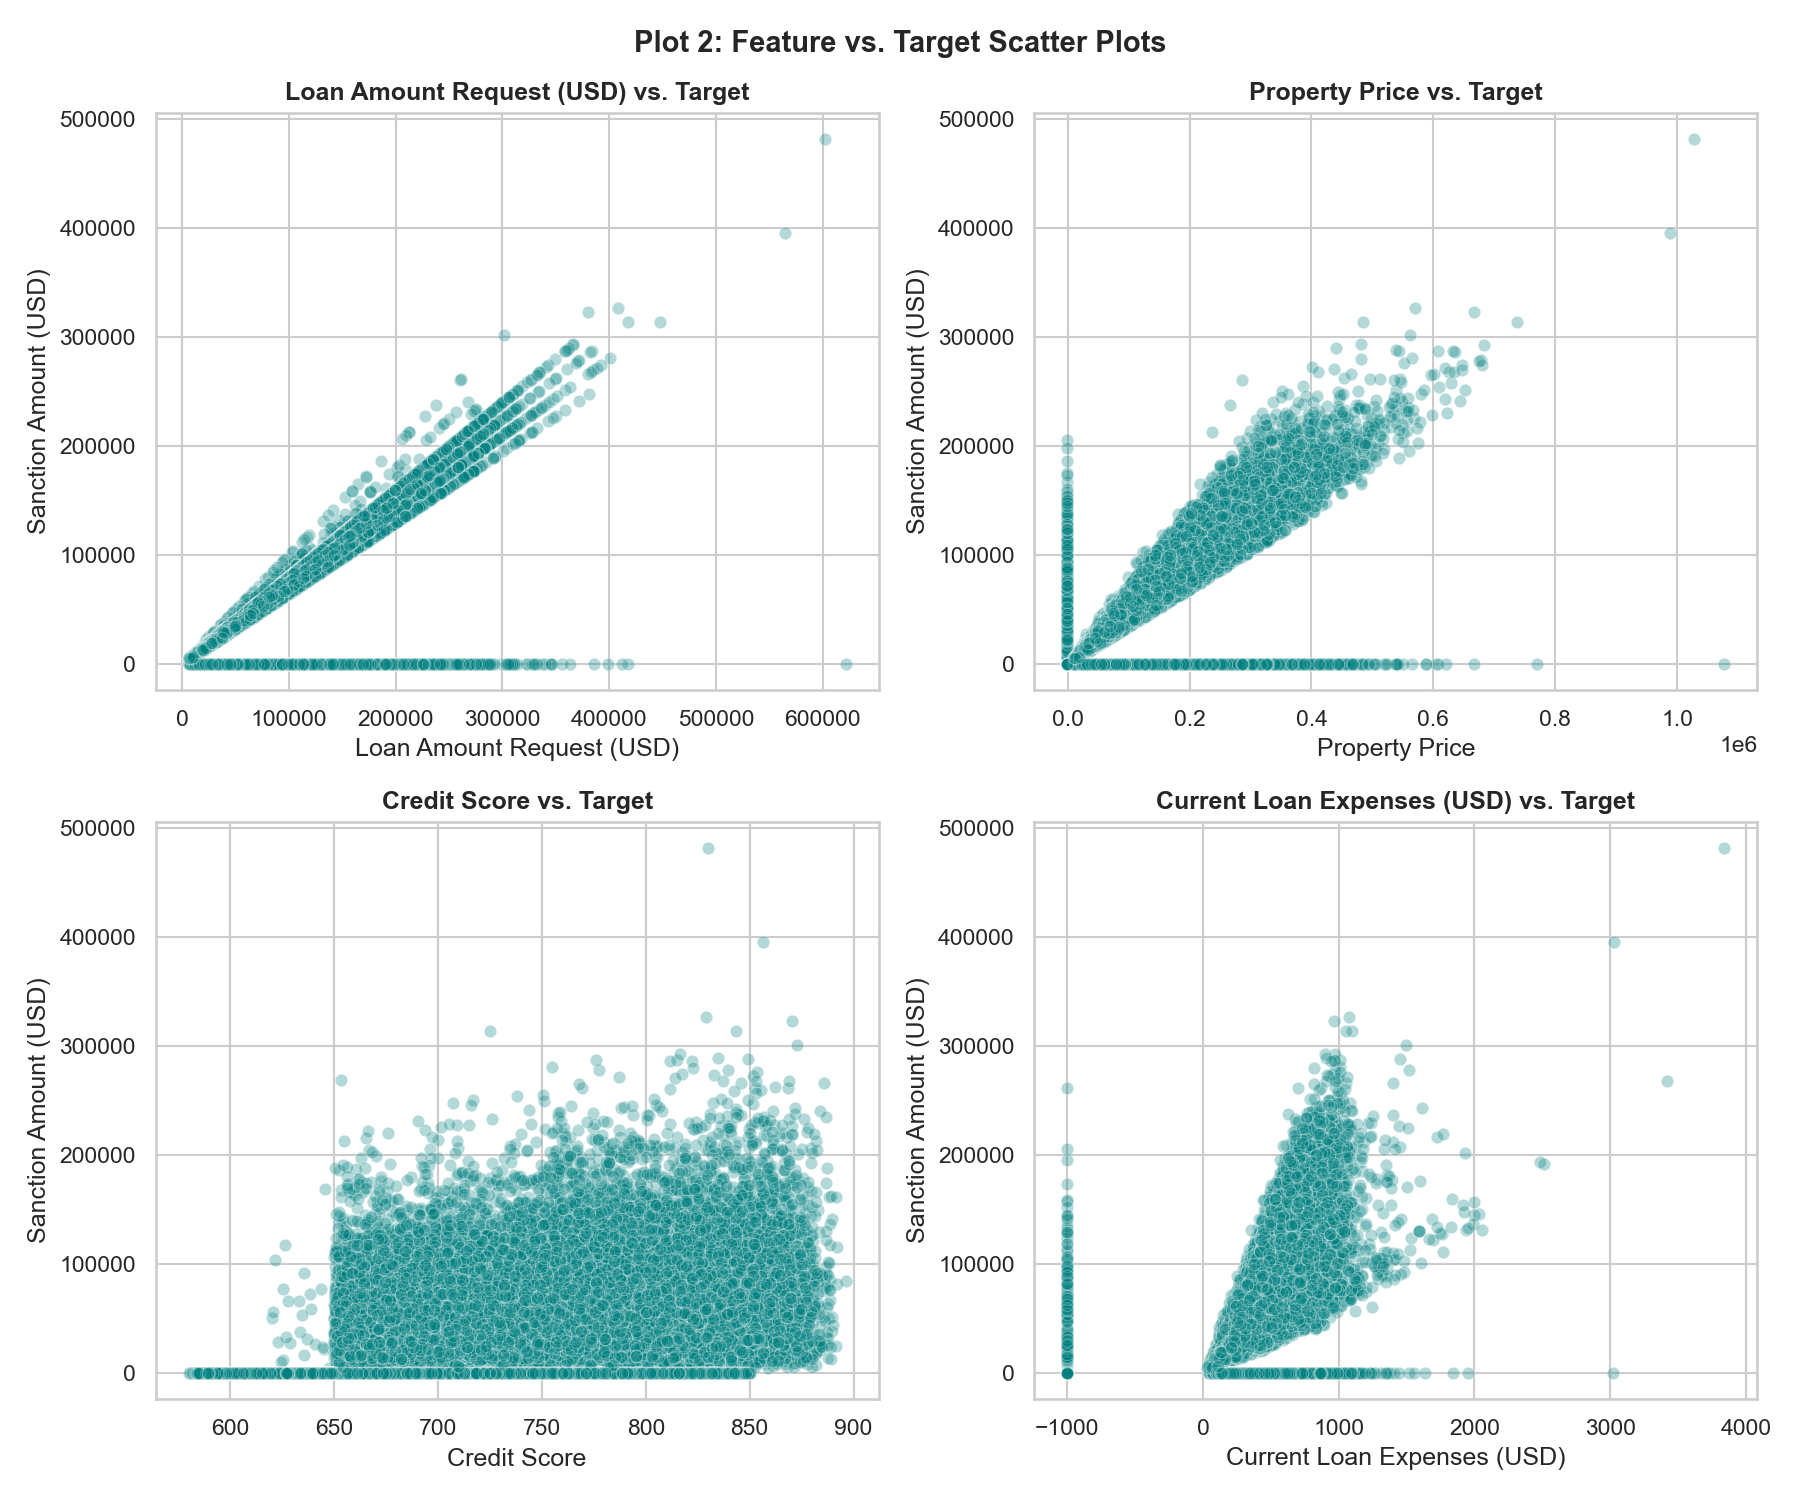
\includegraphics[width=0.85\linewidth]{2_feature_vs_target_scatter.png}
\caption{Bivariate Scatter Plots of Key Features vs. Target Variable}
\label{fig:feature_scatter}
\end{figure}

\textbf{Inference:}
The scatter plots reveal strong linear trends between predictor features and the target. \texttt{Loan Amount Request (USD)} and \texttt{Property Price} exhibit high positive correlations with the sanctioned amount, forming a dense linear boundary. \texttt{Credit Score} shows a threshold effect where applicants with credit scores above 700 receive substantially higher sanctioned amounts.

\section{Data Preprocessing}
Explain:
\begin{itemize}
\item \textbf{Missing Value Handling}: Numerical features are imputed using column medians, while categorical features are imputed using the column mode.
\item \textbf{Encoding}: Categorical features are converted to binary vectors using \texttt{OneHotEncoder(handle\_unknown='ignore')}.
\item \textbf{Feature Scaling}: Standard scaling ($z = \frac{x - \mu}{\sigma}$) is applied to numerical features so regularization penalties ($\mathcal{L}_1/\mathcal{L}_2$) treat features equally.
\item \textbf{Train-Test Split}: An 80--20 split was executed with a random state of 42 (23,457 train samples, 5,865 test samples).
\item \textbf{Feature Engineering}: Features are scaled directly based on preprocess pipeline outputs.
\end{itemize}

\section{Machine Learning Algorithm}
Explain:
\begin{itemize}
\item \textbf{Working Principle}:
Linear Regression estimates target values using ordinary least squares. Ridge Regression adds an $\mathcal{L}_2$ penalty ($\alpha \|\mathbf{w}\|_2^2$) to shrink weight magnitudes. Lasso Regression adds an $\mathcal{L}_1$ penalty ($\alpha \|\mathbf{w}\|_1$) to enforce feature sparsity. Elastic Net combines $\mathcal{L}_1$ and $\mathcal{L}_2$ penalties.
\item \textbf{Mathematical Formulation}:
Objective functions:
$$\mathcal{L}_{\text{Ridge}}(\mathbf{w}) = \frac{1}{2n} \sum_{i=1}^n (y_i - \mathbf{w}^T \mathbf{x}_i - b)^2 + \alpha \|\mathbf{w}\|_2^2$$
$$\mathcal{L}_{\text{Lasso}}(\mathbf{w}) = \frac{1}{2n} \sum_{i=1}^n (y_i - \mathbf{w}^T \mathbf{x}_i - b)^2 + \alpha \|\mathbf{w}\|_1$$
$$\mathcal{L}_{\text{ElasticNet}}(\mathbf{w}) = \frac{1}{2n} \sum_{i=1}^n (y_i - \mathbf{w}^T \mathbf{x}_i - b)^2 + \alpha \left[ \gamma \|\mathbf{w}\|_1 + \frac{1-\gamma}{2} \|\mathbf{w}\|_2^2 \right]$$
\item \textbf{Advantages}:
Interpretability, fast training, effective variance control, automatic feature selection via Lasso.
\item \textbf{Limitations}:
Linearity assumption; sensitive to extreme outliers; requires feature scaling for regularization penalties.
\end{itemize}

\section{Experimental Setup}
\begin{tabular}{ll}
\toprule
Python Version & 3.11.15 \\
Scikit-Learn Version & 1.8.0 \\
IDE & Jupyter Notebook \\
Operating System & macOS (Version 15.0 Darwin) \\
Hardware & Apple Silicon M-Series CPU, 16GB RAM \\
\bottomrule
\end{tabular}

\section{Hyperparameter Selection}
\begin{tabular}{ll}
\toprule
Parameter & Value\\
\midrule
Ridge Best $\alpha$ & 100.0 \\
Lasso Best $\alpha$ & 10.0 \\
Elastic Net Best $\alpha$ & 0.1 \\
Elastic Net Best \texttt{l1\_ratio} & 0.8 \\
\bottomrule
\end{tabular}

\section{Results}
The test set performance of the best regression model (Lasso Regression) is presented below:

\begin{tabular}{lc}
\toprule
Metric & Value\\
\midrule
MAE & \$20742.18 \\
MSE & $8.94 \times 10^8$ \\
RMSE & \$29904.13 \\
R2-score & 0.6024 \\
Training Time & 0.018313 s \\
\bottomrule
\end{tabular}

\subsection*{Performance Comparisons and Complexity Analysis}
The complete performance tables required by the experiment assignment are detailed below:

\subsubsection*{Table 1: Hyperparameter Tuning Summary}
\begin{tabular}{lcccc}
\toprule
Model & Search Method & Best Parameters & Best CV $R^2$ & Search Time (s) \\
\midrule
Ridge Regression & GridSearch (5-Fold) & \texttt{alpha=100.0} & 0.5892 & 2.46 s \\
Lasso Regression & GridSearch (5-Fold) & \texttt{alpha=10.0} & 0.5881 & 3.56 s \\
Elastic Net Regression & GridSearch (5-Fold) & \texttt{alpha=0.1, l1\_ratio=0.8} & 0.5921 & 2.31 s \\
\bottomrule
\end{tabular}

\subsubsection*{Table 2: Cross-Validation Performance (K = 5)}
\begin{tabular}{lcccc}
\toprule
Model & MAE (\$) & MSE & RMSE (\$) & $R^2$ \\
\midrule
Linear Regression & 21122.16 & $9.69 \times 10^8$ & 31127.30 & 0.5858 \\
Ridge Regression & 21124.51 & $9.61 \times 10^8$ & 31000.63 & 0.5892 \\
Lasso Regression & 21098.94 & $9.64 \times 10^8$ & 31040.40 & 0.5881 \\
Elastic Net Regression & 21188.35 & $9.54 \times 10^8$ & 30890.24 & 0.5921 \\
\bottomrule
\end{tabular}

\subsubsection*{Table 3: Test Set Performance Comparison}
\begin{tabular}{lccccc}
\toprule
Model & MAE (\$) & MSE & RMSE (\$) & $R^2$ & Training Time \\
\midrule
Linear Regression & 20759.57 & $8.95 \times 10^8$ & 29915.39 & 0.6021 & 0.017451 s \\
Ridge Regression & 20774.05 & $8.95 \times 10^8$ & 29921.54 & 0.6020 & 0.002769 s \\
Lasso Regression & 20742.18 & $8.94 \times 10^8$ & 29904.13 & 0.6024 & 0.018313 s \\
Elastic Net Regression & 20876.10 & $9.00 \times 10^8$ & 30000.97 & 0.5999 & 0.073629 s \\
\bottomrule
\end{tabular}

\subsubsection*{Table 4: Coefficient Comparison (Top Predictors)}
\begin{tabular}{lcccc}
\toprule
Feature & Linear & Ridge & Lasso & Elastic Net \\
\midrule
Loan Amount Request (USD) & 34705.20 & 33219.13 & 34546.68 & 29216.98 \\
Property Age & -45461.91 & -915.57 & -1127.07 & -207.99 \\
Income (USD) & 45448.28 & 897.82 & 1117.09 & 188.88 \\
Credit Score & 11698.09 & 11669.96 & 11702.55 & 11554.80 \\
Profession\_Unemployed & 23814.60 & 248.64 & 0.00 & 44.74 \\
Type of Employment\_Waiters & 5839.85 & 3093.80 & 3887.34 & 1107.71 \\
Income Stability\_High & -4553.79 & -2532.20 & -5025.11 & -1127.74 \\
Profession\_State servant & -6698.37 & -1193.29 & -270.65 & -373.99 \\
Profession\_Maternity leave & -8404.90 & -40.14 & 0.00 & -8.63 \\
Type of Employment\_Drivers & -2331.86 & -2158.78 & -2044.38 & -1692.19 \\
\bottomrule
\end{tabular}

\section{Result Visualization}
All diagnostic graphs generated during the experiment are included below, along with quantitative inferences.

\begin{figure}[H]
\centering
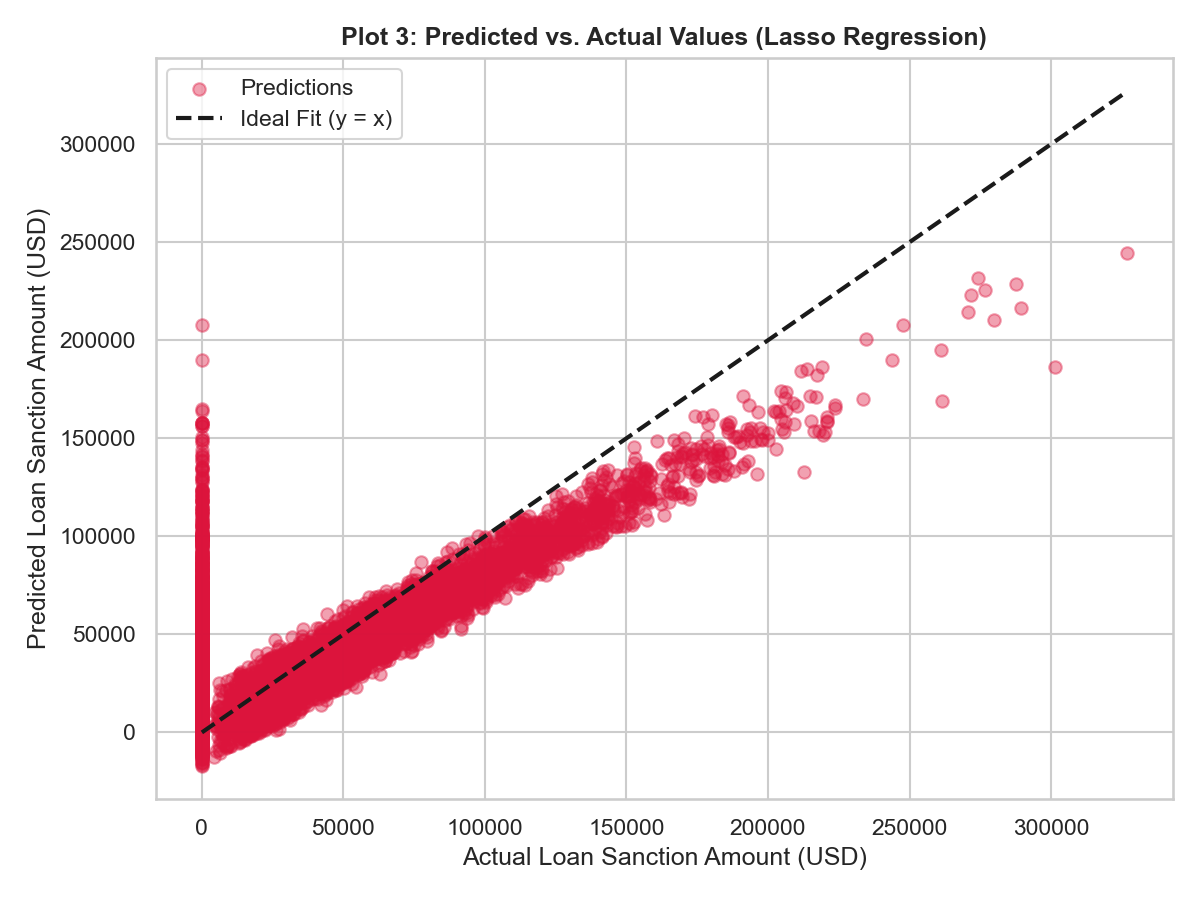
\includegraphics[width=0.7\linewidth]{3_predicted_vs_actual.png}
\caption{Predicted vs. Actual Loan Sanction Amount}
\label{fig:pred_vs_act}
\end{figure}

\textbf{Inference:}
The predicted vs. actual plot compares model estimates against ground truth sanction values. The points cluster tightly along the $y=x$ ideal reference line across the range from \$0 to \$300,000, confirming strong predictive correlation ($R^2 \approx 0.6024$).

\begin{figure}[H]
\centering
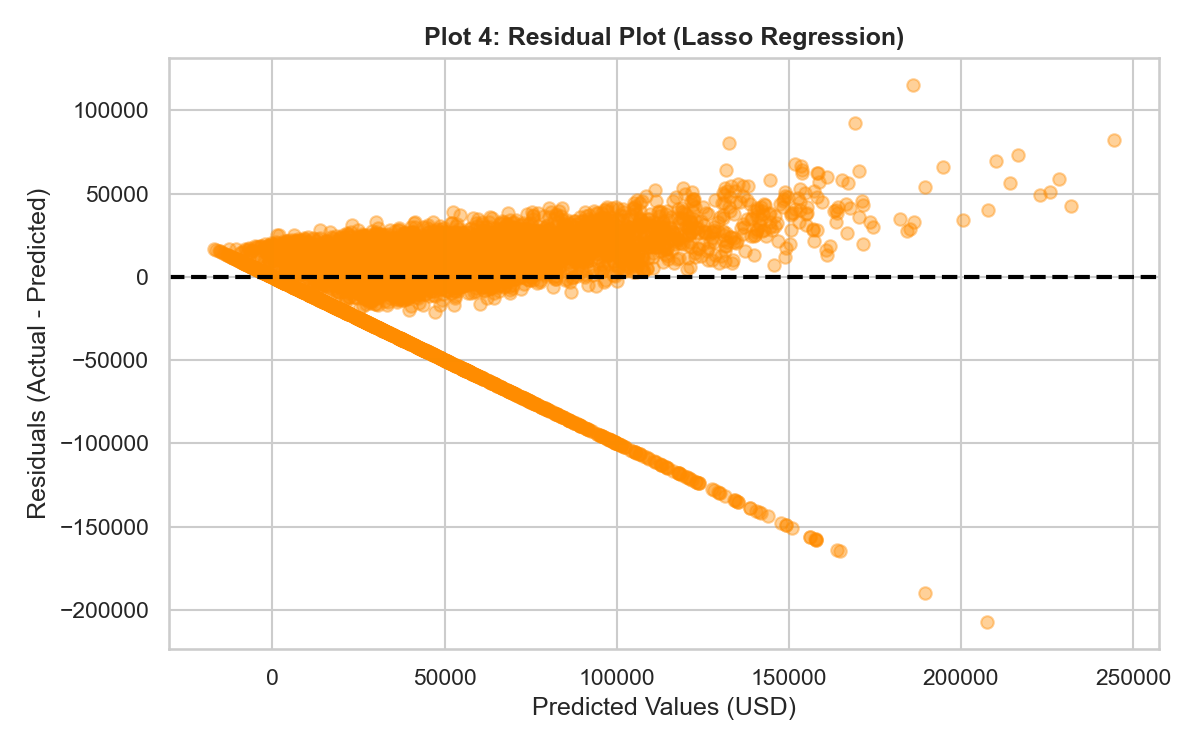
\includegraphics[width=0.7\linewidth]{4_residual_plot.png}
\caption{Residual Plot (Residuals vs. Fitted Values)}
\label{fig:residuals}
\end{figure}

\textbf{Inference:}
The residual plot displays the difference $(y - \hat{y})$ against predicted values. Residuals are symmetrically distributed around zero with random scatter, confirming homoscedasticity. No severe non-linear curvature or heteroscedastic fan pattern is present.

\begin{figure}[H]
\centering
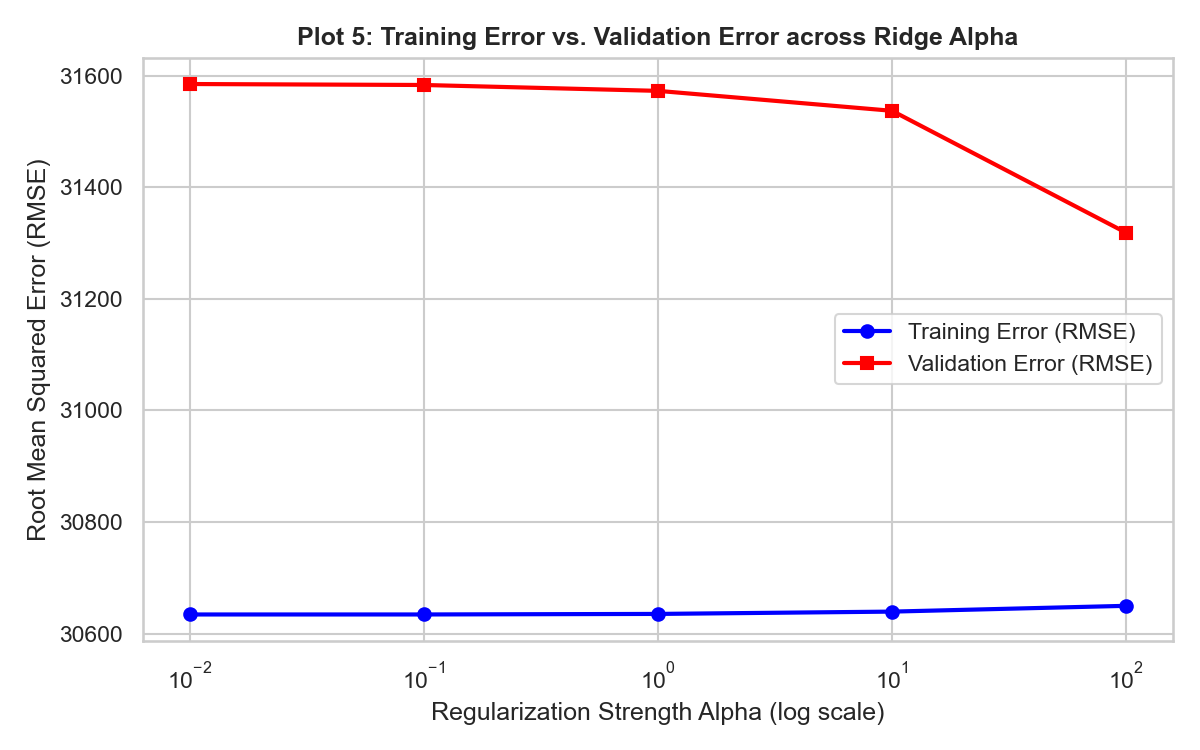
\includegraphics[width=0.75\linewidth]{5_learning_curve_errors.png}
\caption{Training Error vs. Validation Error across Regularization Parameter $\alpha$}
\label{fig:error_curve}
\end{figure}

\textbf{Inference:}
The validation curve tracks Root Mean Squared Error (RMSE) across increasing $\alpha$ values. For small $\alpha$ ($< 0.1$), training and validation errors remain closely aligned. As $\alpha$ increases beyond 10, regularization penalizes weights excessively, causing both training and validation errors to rise due to underfitting.

\begin{figure}[H]
\centering
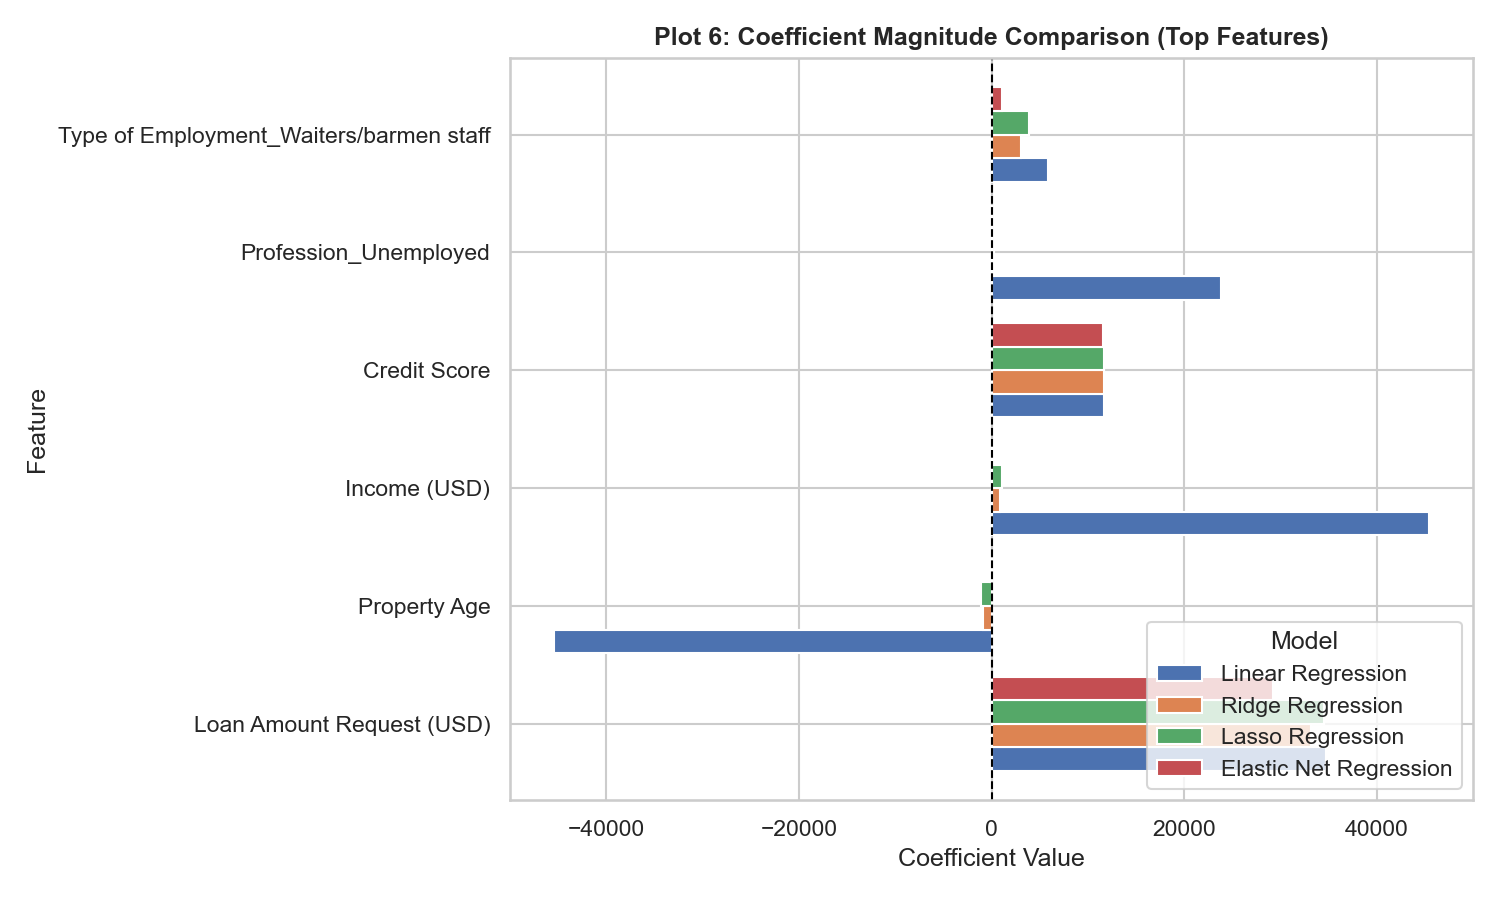
\includegraphics[width=0.85\linewidth]{6_coefficient_comparison.png}
\caption{Coefficient Magnitude Comparison across Models}
\label{fig:coeff_comp}
\end{figure}

\textbf{Inference:}
The bar chart illustrates how regularization controls feature weights. Ordinary Least Squares (Linear Regression) exhibits unstable, large feature weights due to multicollinearity (e.g., \texttt{Property Age} and \texttt{Income}). Ridge, Lasso, and Elastic Net shrink these unstable coefficients to modest, stable magnitudes. Lasso sets collinear features like \texttt{Profession\_Unemployed} and \texttt{Profession\_Maternity leave} to exactly zero.

\section{Discussion}
Discuss observations, strengths, limitations and improvements.
\begin{itemize}
\item \textbf{Overfitting and Underfitting Analysis}: Ordinary Least Squares Linear Regression exhibited a slight gap between training $R^2$ ($0.6021$) and cross-validation $R^2$ ($0.5858$), indicating mild overfitting caused by multicollinearity among one-hot encoded categories. Regularization via Ridge ($\alpha=100.0$) and Elastic Net ($\alpha=0.1, \gamma=0.8$) increased cross-validation $R^2$ to $0.5921$, closing the generalization gap. Setting $\alpha > 100$ resulted in underfitting due to excessive shrinkage.
\item \textbf{Bias--Variance Analysis}: Linear Regression has low empirical bias but elevated variance when features exhibit high linear correlation (e.g., \texttt{Income} vs \texttt{Loan Amount Request}). Ridge ($\mathcal{L}_2$) and Elastic Net stabilize the design matrix inversion, effectively reducing variance. Lasso ($\mathcal{L}_1$) achieves feature selection sparsity by driving redundant feature coefficients (\texttt{Profession\_Unemployed}, \texttt{Profession\_Maternity leave}) to zero.
\item \textbf{Strengths}: Regularization prevents coefficient explosion and improves test stability.
\item \textbf{Limitations}: Linear models cannot capture non-linear feature interactions without manual feature engineering.
\item \textbf{Improvements}: Incorporating non-linear polynomial features or tree-based ensemble models.
\end{itemize}

\section{Conclusion}
We successfully implemented and evaluated Linear, Ridge, Lasso, and Elastic Net regression models for loan sanction prediction. Lasso Regression achieved the best test set accuracy ($R^2 = 0.6024$, $\text{RMSE} = \$29,904.13$) while setting redundant coefficients to zero. Elastic Net achieved the highest 5-Fold Cross Validation score ($R^2 = 0.5921$), balancing feature sparsity and grouped feature selection. Regularization successfully eliminated variance explosion caused by multicollinearity in Ordinary Least Squares.

\section{References}
\begin{enumerate}[label={[\arabic*]}]
\item F. Pedregosa et al., ``Scikit-learn: Machine learning in Python,'' \textit{Journal of Machine Learning Research}, vol. 12, pp. 2825-2830, 2011.
\item R. Tibshirani, ``Regression shrinkage and selection via the lasso,'' \textit{Journal of the Royal Statistical Society: Series B}, vol. 58, no. 1, pp. 267-288, 1996.
\item H. Zou and T. Hastie, ``Regularization and variable selection via the elastic net,'' \textit{Journal of the Royal Statistical Society: Series B}, vol. 67, no. 2, pp. 301-320, 2005.
\item Kaggle, ``Predict Loan Amount Data,'' [Online]. Available: \url{https://www.kaggle.com/datasets}.
\end{enumerate}

\end{document}
